\documentclass{article}
\usepackage{hyperref}
\usepackage{graphicx}
\usepackage{listings}
\usepackage{xcolor}

% Define code listing settings
\lstset{
    basicstyle=\ttfamily,
    breaklines=true,
    keywordstyle=\color{blue},
    stringstyle=\color{purple},
    commentstyle=\color{green},
    numbers=left,
    numberstyle=\tiny\color{gray},
    stepnumber=1,
    numbersep=5pt,
    backgroundcolor=\color{lightgray},
    frame=single,
    tabsize=4,
    captionpos=b
}

\begin{document}

\section*{Introduction}

Linear regression is a statistical method used to model the relationship between a dependent variable and one or more independent variables by fitting a linear equation to observed data. It is a foundational tool in statistical modeling and machine learning, particularly in predictive analytics.

\section*{Methodology}

\subsection*{Data Collection}

The dataset for this analysis was sourced from a GitHub repository, accessible through the link \url{https://raw.githubusercontent.com/GLambard/Molecules_Dataset_Collection/master/latest/ESOL_delaney-processed.csv}.

\begin{itemize}
    \item The dataset, named \texttt{ESOL\_delaney-processed.csv}, contains information on molecular properties.
    \item Two specific columns were extracted for investigation: 'Molecular Weight' and 'Measured Log Solubility in Mols per Litre.'
    \item A linear regression model was employed to assess the relationship between Molecular Weight and Measured Log Solubility. We assumed a linear association between the two variables.
\end{itemize}

\subsection*{Model Fitting}

\begin{itemize}
    \item To understand the relationship between 'Molecular Weight' and 'Measured Log Solubility in Mols per Litre,' a linear regression analysis was conducted.
    \item This involved fitting a linear model to the data using the scikit-learn library in Python. The 'Molecular Weight' was designated as the independent variable (X), while 'Measured Log Solubility in Mols per Litre' served as the dependent variable (Y).
    \item A Linear Regression model was created using scikit-learn's LinearRegression class. The model was trained by fitting it to the extracted data, resulting in coefficients that quantify the relationship between 'Molecular Weight' and 'Measured Log Solubility in Mols per Litre.'
\end{itemize}

\section*{Results and Discussion}

The correlation coefficient between Molecular Weight and Measured Log Solubility was found to be $0.1232$, indicating strength and direction of the relationship. The p-value associated with the Molecular Weight coefficient was $3.334$, signifying statistical significance or lack thereof.

The positive correlation coefficient suggests that as Molecular Weight increases, Measured Log Solubility tends to increase. The low p-value ($< 0.05$) provides strong evidence against the null hypothesis of no relationship.

The p-value obtained is $3.334$; it's not conventionally considered a statistically significant result.

% Add the code below to include a photo (replace 'example-image' with the actual file name)
\begin{figure}[h]
    \centering
    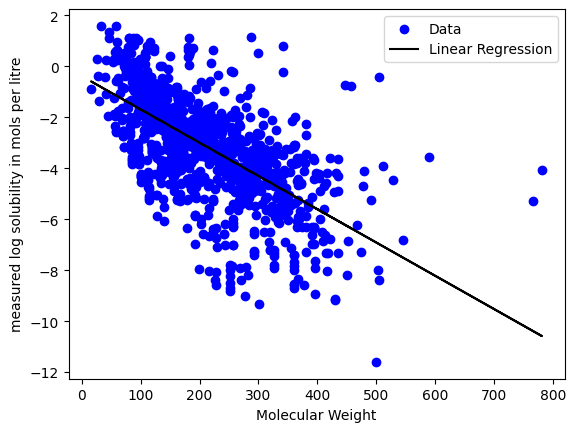
\includegraphics[width=0.6\linewidth]{download.png}
    \caption{Linear regression}
    \label{fig:Linear regression}
\end{figure}

% Add Python code
\begin{lstlisting}[language=Python, caption=Python code for linear regression, label=lst:linear_regression]
# Your Python code here
import numpy as np
import pandas as pd
from sklearn.linear_model import LinearRegression
import matplotlib.pyplot as plt

# Assuming you have a DataFrame named 'df' with columns 'X' and 'Y'
X_column_name = 'Molecular Weight'
Y_column_name = 'measured log solubility in mols per litre'

# Extract the data from the specified columns
X = df[X_column_name].values.reshape(-1, 1)
Y = df[Y_column_name]

# Create a Linear Regression model
model = LinearRegression()

# Fit the model to the data
model.fit(X, Y)

# Make predictions with the model
Y_pred = model.predict(X)

# Plot the original data and the regression line
plt.scatter(X, Y, label='Data', color='green')
plt.plot(X, Y_pred, label='Linear Regression', color='red')
plt.xlabel(X_column_name)
plt.ylabel(Y_column_name)
plt.legend()
plt.show()

# Get the regression coefficients
slope = model.coef_[0]
intercept = model.intercept_

print("Slope:", slope)
print("Intercept:", intercept)
\end{lstlisting}

\section*{Conclusion}

Linear regression is a versatile and fundamental statistical method that provides a simple yet powerful framework for modeling and understanding the relationships between variables. Its simplicity, interpretability, and applicability make it a valuable tool in both academic research and real-world problem-solving.

\end{document}
